\RequirePackage[T1]{fontenc}
\documentclass[conference]{IEEEtran}
\usepackage{graphicx,booktabs,amsmath,url}
\usepackage[hidelinks]{hyperref}
\title{Neuro-Symbolic Causal Inference:\\DistilBERT and Reviewed Bayesian Graphs}
\author{\IEEEauthorblockN{Aman, Ansh Tomar, Ravleen Singh, Ritik, and Sarabjeet Singh}
\IEEEauthorblockA{CSAI Advanced Machine Learning and Deep Learning Project\\Phase 2: Local Compute-Budget Evaluation}}
\begin{document}
\maketitle
\begin{abstract}
We extend a classical machine-learning causal-claim baseline with a compact transformer and an explicitly reviewed graph stage. A shared DistilBERT encoder reads complete premise--hypothesis examples through token windows; their representations are averaged before a document-level classification decision. We compare frozen and fine-tuned encoders, ordinary and class-weighted loss, and a fixed average of ML and DL scores. All budget-matched models train on 2100 examples from 25 whole premise groups. Evaluation uses 984 development examples and the official 1,162-example test split. Graph evaluation targets entailed direct relations on 18 complete-pair test systems, rather than claiming recovery of a full hidden causal DAG. Separately, specified conditional probability distributions permit numerically checked intervention examples. Results are limited to one seed, a small training subset, and synthetic template language; we make no claim of real-world causal discovery.
\end{abstract}
\begin{IEEEkeywords}
causal reasoning, DistilBERT, neuro-symbolic inference, Bayesian networks, ablation study
\end{IEEEkeywords}

\section{Problem and Phase 1 Baseline}
A causal hypothesis may sound plausible without following from statistical premises. Corr2Cause asks whether a causal claim is entailed by a closed-system description of correlations and independences~\cite{corr}. Label 1 means entailed; label 0 means not entailed, which is not equivalent to impossibility in every compatible graph. The task is binary reasoning over supplied hypotheses, not unrestricted extraction from scientific articles.

The corrected Phase 1 implementation uses 28 handcrafted features, Logistic Regression, a linear SVM and a Random Forest. Its calibrated full-data Random Forest reaches macro F1 0.6357. That baseline trains on 205,734 records and is contextual evidence only when compared with the much smaller Phase 2 budget. We retain the original submission separately and do not silently replace historical results.

The Phase 2 research questions are: (1) whether task-specific transformer fine-tuning improves on frozen representations and budget-matched ML, (2) whether class weighting helps, (3) whether combining structural and text scores adds value, and (4) how graph consistency checks affect entailed-edge quality.

\section{Data and Evaluation Protocol}
The official CSVs contain 205,734 training, 1,076 development and 1,162 test records. File hashes and the pinned dataset revision are retained in the project. Development examples sharing a premise with training or test are excluded from selection, leaving 984 examples. Test labels do not choose checkpoints, thresholds, model family or demonstration cases. The test split was already observed during Phase 1, so this is a fixed-protocol evaluation rather than a previously untouched benchmark.

A warmed Apple GPU pilot motivated a local compute budget. We shuffle training premise groups with seed 42 and retain whole groups until reaching the configured row budget. The resulting sample has 2100 examples from 25 systems, with 332 positive labels. Every budget-matched model uses exactly these sample IDs. Preserving groups avoids splitting different hypotheses about one system across derived training partitions. The sample is not claimed to represent the full dataset distribution. The complete sample manifest is saved.

\subsection{Long Examples}
A read-only word-count audit found 50,589 training records above 512 whitespace words. Word counts are not tokenizer counts. We therefore measure exact token lengths and never silently truncate. Within the selected data, 4 training windows are needed at most; 810 training rows use multiple windows. Each test pair fits in one window under the pinned tokenizer. This train--test length difference is a limitation.

\section{Model Architecture}
We use the pinned \texttt{distilbert-base-uncased} checkpoint, a distilled BERT encoder~\cite{bert,distil}. Self-attention computes
\begin{equation}
\operatorname{Attention}(Q,K,V)=\operatorname{softmax}(QK^T/\sqrt{d_k})V.
\end{equation}
The checkpoint has six encoder layers, 12 attention heads and hidden dimension 768. Bidirectional attention relates premise and hypothesis tokens within a window. Its attention weights are not causal graph edges. We fine-tune an already distilled model; we do not perform teacher--student distillation ourselves.

Each window contains a consecutive premise segment and the complete hypothesis, plus special tokens, within 512 positions. The same encoder parameters process all windows. If $h_{ij}$ is the first-token representation of window $j$ for example $i$, the document vector is
\begin{align}
\bar h_i&=\frac{1}{K_i}\sum_{j=1}^{K_i}h_{ij},\\
p_i&=\operatorname{softmax}(W_2\operatorname{ReLU}(W_1\bar h_i+b_1)+b_2).
\end{align}
Dropout of 0.2 is applied in the classification head. Token tensors are padded to 512 positions with attention masks. Fixed padding and bounded device-cache handling avoid excessive Apple GPU graph caching; neither removes valid input tokens. Flattening valid windows means padded document windows cannot affect pooling. We compute one loss for each original document; global document labels are not assigned independently to every partial window. Averaging preserves token coverage but does not allow full cross-window attention, so it is not a proof of multi-step logical reasoning.

\subsection{Optimization and Regularization}
The main encoder is fine-tuned with AdamW, learning rate $2\times10^{-5}$, weight decay 0.01, gradient clipping at norm 1, and up to three epochs. Document batch size is two, with eight accumulation steps where available. Early stopping uses one epoch without improvement in development macro F1. Candidate thresholds span 0.05 to 0.95; development macro F1 chooses the threshold with a fixed higher-threshold tie rule. We retain the best checkpoint.

Weighted cross entropy uses training class counts: $w_c=N/(2N_c)$. The ordinary-loss ablation removes these weights while retaining the fine-tuning protocol. The frozen-encoder baseline caches document vectors and trains its head with learning rate 0.001 and batch size 64. This is an efficient feature-based comparator; the different head optimization means it is not a perfectly controlled single-variable comparison. All required runs use seed 42 and float32. Fine-tuning uses Apple MPS; the frozen encoder is evaluated on CPU in parallel with GPU work. Timings therefore reflect different devices and are not a hardware-controlled speed comparison. We do not report unperformed seed repetitions or unmeasured significance.

\subsection{Matched ML and Hybrid Scores}
The matched baseline is a depth-10, 100-tree Random Forest with balanced classes and three-fold training-only sigmoid calibration. It uses the existing 28 features and the identical training sample. We also test a fixed score average,
\begin{equation}
s_{hybrid}=\tfrac12s_{ML}+\tfrac12p_{DL}.
\end{equation}
The rationale is potentially complementary structural features and learned text representations. No meta-model is trained. Scores sharing a numeric range are not automatically calibrated; measured development/test behavior is the evidence. Demonstration model selection is committed using development results before test metrics are computed. A hybrid bonus or improved performance is not assumed.

\section{Graph Construction and Independent Review}
Each premise defines its own anonymous variable system. Only explicit direct-cause hypotheses become directed candidate edges. Ancestor, collider and confounder claims remain typed annotations; an unnamed common cause does not justify an edge between its effects. Self-loops are rejected. Cycle handling removes the minimum-score edge in each discovered cycle, with deterministic lexical tie-breaking. It enforces acyclicity, not causal truth. D-separation reads conditional independence from the graph: conditioning on the middle node blocks a chain or fork, while a collider blocks a path unless it or a descendant is conditioned on. These rules justify the stated small-system review assumptions~\cite{pearl}.

\subsection{Reference Edges}
We identify 18 test systems whose annotations cover all ordered non-self direct-cause variable pairs. Label-1 pairs define a reference graph of entailed direct relations. Label-0 pairs are not entailed and need not be impossible in every generating DAG. Eleven systems contain positive reference edges; seven contain none. All 18 remain in pooled TP/FP/FN accounting. We report precision, recall, edge F1, system coverage and removed-edge counts before and after cycle handling. No-edge precision is undefined rather than presented as perfect.

\subsection{Label-Blind Demonstration Review}
For small development systems with at most six variables, a deterministic reviewer first derives the adjacency skeleton from separating sets and then enumerates compatible edge directions under closed-system, acyclicity, causal Markov, faithfulness and complete-independence-description assumptions. A proposed edge is approved only when every compatible DAG contains it; unsupported or ambiguous claims are rejected or marked uncertain. For these fully specified small systems the logical audit can resolve claims without a neural model; it is a validation aid, not evidence that DL is necessary. This code reads premises and proposed edges, not reference labels. It is automated logical review, not human approval, and is used only for the demonstration, not to edit the automatic test scores.

\section{Bayesian Queries and Assumptions}
A Bayesian model factorizes as
\begin{equation}
P(v)=\prod_i P(v_i\mid \operatorname{Pa}(v_i)).
\end{equation}
Under a causal interpretation, setting $X=x$ replaces its mechanism and removes its factor in the truncated product. This differs from merely conditioning on an observed value. A graph alone does not determine numerical causal effects. The integration demo supplies explicit binary CPDs for its approved graph, checks model consistency and compares an intervention query with independent enumeration of the truncated factorization. Integration graph source: Hybrid matched ML + DL.  The reviewed graph was passed to pgmpy with supplied CPDs. The query P(D=1 | do(A=1)) returned 0.6000, agreeing with independent enumeration (0.6000).

A separate specified confounded network has edges $Z\rightarrow X$, $Z\rightarrow Y$, and $X\rightarrow Y$. Its documented CPDs yield $P(Y=1\mid X=1)=0.89$, $P(Y=1\mid do(X=1))=0.85$, and $P(Y=1\mid do(X=0))=0.25$. We verify these numerically. These probabilities are supplied demonstration assumptions, not empirical mechanisms estimated from Corr2Cause. Numerical queries without explicit CPDs are refused. Individual counterfactual estimation is outside the implemented scope.

\section{Measured Results}
\begin{table}[t]
\caption{Classifier comparison; P/R refer to the positive class. *Full-data RF uses a different training budget.}
\centering\scriptsize
\begin{tabular}{lrrrr}\toprule
Model & Dev F1 & Test F1 & P & R\\\midrule
Matched RF & 0.5788 & 0.5927 & 0.3431 & 0.2611 \\
Frozen encoder & 0.5917 & 0.5679 & 0.3040 & 0.2111 \\
Fine-tuned DL & 0.6844 & 0.6726 & 0.3739 & 0.7333 \\
Ordinary loss & 0.6510 & 0.6443 & 0.3408 & 0.6722 \\
ML + DL average & 0.6871 & 0.6718 & 0.3725 & 0.7389 \\
Full-data RF* & 0.6534 & 0.6357 & 0.3510 & 0.4778 \\
\bottomrule\end{tabular}
\label{tab:class}
\end{table}
The model selected for the demonstration by development macro F1 is Hybrid matched ML + DL. The primary fine-tuned model's test macro F1 is 0.6726; the fixed hybrid achieves 0.6718. In this run, the average did not improve held-out macro F1 over DL alone, despite its slightly higher development score. We retain the development-selected demonstration model rather than switching based on test results. These are measured results on a small sample, not evidence that adding deep learning necessarily improves causal reasoning. Table~\ref{tab:class} includes both positive-class metrics and macro F1 to avoid accuracy-only conclusions under imbalance.

\begin{figure}[t]
\centering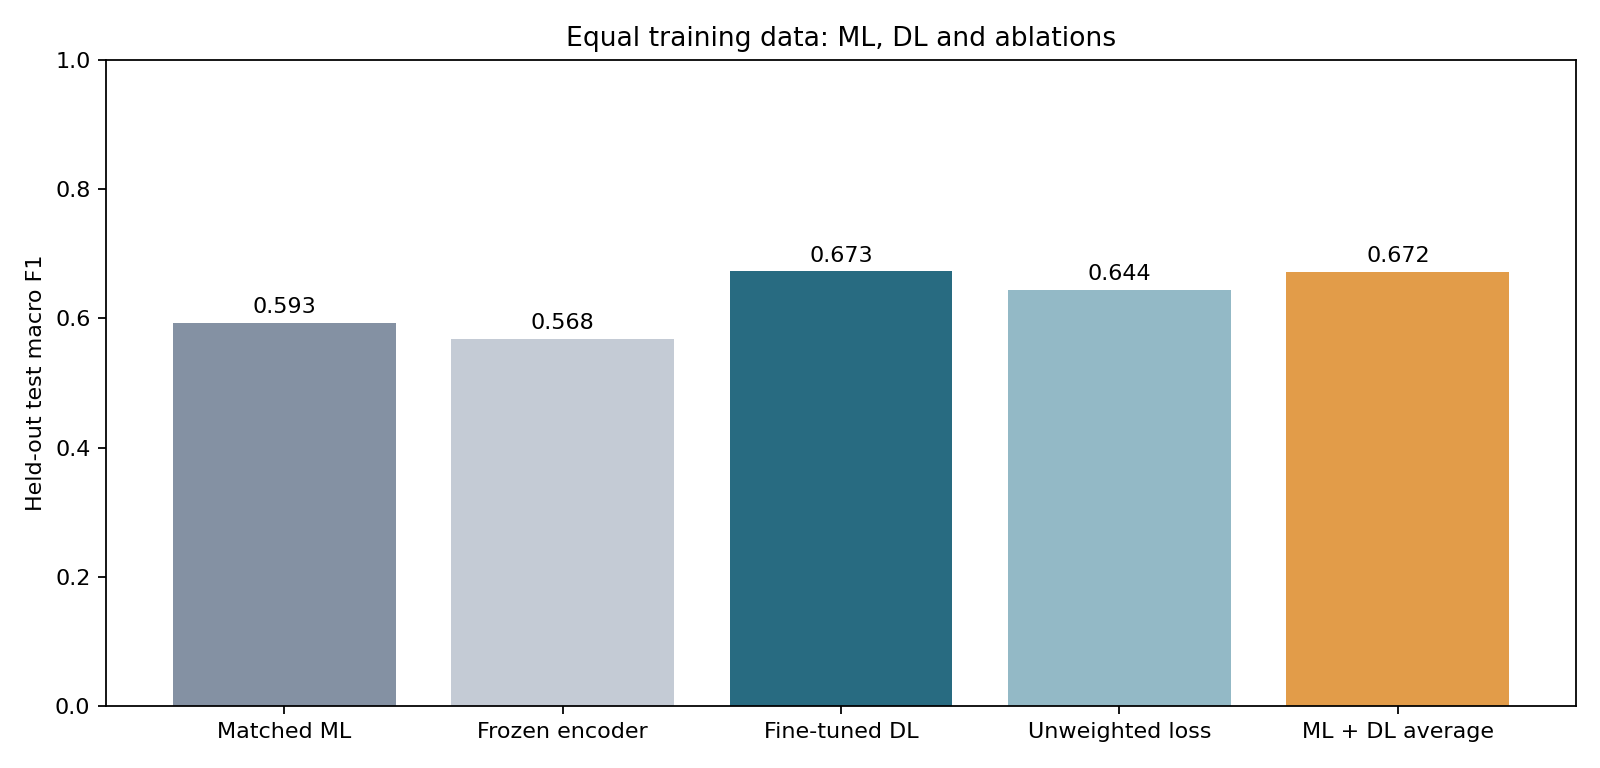
\includegraphics[width=\columnwidth]{../../results/phase2/classification.png}
\caption{Budget-matched classification and ablation results. All displayed models use the same sampled training records.}
\end{figure}

\begin{table}[t]
\caption{Entailed-edge evaluation on 18 complete-pair systems. Precision before/after cycle handling, recall after, and removed edges.}
\centering\scriptsize
\begin{tabular}{lrrrr}\toprule
Model & P before & P after & R after & Removed\\\midrule
Matched RF & -- & -- & 0.0000 & 0 \\
Frozen encoder & -- & -- & 0.0000 & 0 \\
Fine-tuned DL & 0.3710 & 0.4167 & 0.7759 & 16 \\
Ordinary loss & 0.5246 & 0.5439 & 0.5345 & 4 \\
ML + DL average & 0.3730 & 0.4128 & 0.7759 & 17 \\
Full-data RF* & 0.2642 & 0.0000 & 0.0000 & 53 \\
\bottomrule\end{tabular}
\end{table}
Cycle removal is evaluated as a structural ablation rather than credited as a classification improvement. It may improve precision, reduce recall, or leave edge quality unchanged. Empty predictions and systems without entailed reference edges remain visible in machine-readable results. Automated reviewed demonstration edges are not substituted into these scores.

\begin{table}[t]
\caption{Local training/validation cost: fine-tuning on MPS; frozen encoder on CPU. Time excludes final test inference.}
\centering\small
\begin{tabular}{lrrr}\toprule
Run & Epochs & Best epoch & Minutes\\\midrule
Weighted DL & 3 & 3 & 13.7 \\
Ordinary loss & 3 & 2 & 12.7 \\
Frozen encoder & 3 & 3 & 4.7 \\
\bottomrule\end{tabular}
\end{table}

\section{Reproducibility and Validation}
The CLI prepares data, trains named experiments, evaluates saved scores and runs the offline demo. Artifacts record model/data revisions, sample IDs, settings, thresholds, epoch histories, weights and source/config fingerprints; stale artifacts are rejected. The notebook reads these files without duplicating model code.

Tests verify token coverage, hypothesis preservation, pooling, label-blind review, graph references, sample isolation, explicit CPDs, checkpoint reloads and numerical query answers. Existing Phase 1 tests remain. The submission includes LaTeX source, the compiled report, an editable deck and an executed notebook.

\section{Limitations and Conclusion}
The principal limitations are the small training budget, one random seed, synthetic template language, limited independent systems, different train/test length distributions, and approximate cross-window pooling. Variable-renaming robustness was not tested, so gains may include template or naming shortcuts. Encoder fine-tuning may fail to outperform the handcrafted baseline. Graph references cover entailed direct edges, not full hidden DAGs; score calibration and causal interpretation are separate questions. The automated reviewer depends on strong stated assumptions and is not a human subject-matter review. CPDs are specified examples, so no empirical real-world effect or counterfactual claim is warranted.

The implementation provides a compact and inspectable DL extension: one encoder, one document decision, one fixed fusion experiment, separate graph evaluation and checked Bayesian inference. The contribution is the reproducible comparison and explicit separation of learned claims, structural consistency and probabilistic assumptions, rather than an unsupported claim of causal discovery.

\begin{thebibliography}{9}
\bibitem{corr} Z. Jin et al., ``Can Large Language Models Infer Causation from Correlation?,'' ICLR, 2024, arXiv:2306.05836.
\bibitem{bert} J. Devlin et al., ``BERT: Pre-training of Deep Bidirectional Transformers for Language Understanding,'' NAACL-HLT, 2019.
\bibitem{distil} V. Sanh et al., ``DistilBERT, a distilled version of BERT: smaller, faster, cheaper and lighter,'' NeurIPS Workshop, 2019, arXiv:1910.01108.
\bibitem{pearl} J. Pearl, \emph{Causality: Models, Reasoning, and Inference}. Cambridge University Press, 2000.
\bibitem{pgmpy} A. Ankan and A. Panda, ``pgmpy: Probabilistic Graphical Models using Python,'' SciPy, 2015.
\end{thebibliography}
\end{document}
